

\section{Experimental setup}
\label{sec:setup}
The analyzed minimum bias events are p--Pb collisions at $\snn$~=~5.02~TeV, which are recorded by the ALICE detector during 2016. The entire subsystem of the ALICE detector is described in \cite{Carminati:2004fp, Abelev:2014ffa} at the LHC Run 2 period. The present analysis is carried out with the V0~\cite{ALICE:2013axi}, the Zero Degree Calorimeter (ZDC)~\cite{Cortese:2019nnv}, the Inner Tracking System (ITS)~\cite{ALICE:2010tia}, the Time-Of-Flight (TOF)~\cite{Jacazio:2018slq}, and the Time Projection Chamber (TPC)~\cite{Alme:2010ke} detectors.

The V0 detector has two stations located at both sides of the interaction point, V0A and V0C, each made of 32 plastic scintillator strips, covering the full azimuthal angle within the pseudorapidity intervals $2.8 < \eta < 5.1$ and $-3.7 < \eta < -1.7$, respectively. For triggering p--Pb collisions, V0A, detector on Pb-going side, is used to provide a minimum bias (MB) trigger. The V0 provides the multiplicity class using the sum of the V0A signals. The collected data samples from the minimum bias trigger corresponds to integrated luminosity of 0.24~nb$^{-1}$~\cite{ALICE:2014gvw}. The ZDC, which detects ``slow'' nucleons at very large $\eta$~\cite{Cortese:2019nnv},  also defines multiplicity class for the event selection.

The primary vertex position is reconstructed using the measured signals in the Silicon Pixel Detector (SPD)~\cite{Santoro2009:ALICESPD}, which is innermost two layers of the ITS. Reconstructed primary vertex is required to be within 10~cm from the center of the detector along the beam direction. The probability of pileup events is 0.5\% in MB events. Pileup events are rejected if the longitudinal displacement of their reconstructed vertices is larger than 0.8~cm. The TPC is the main tracking detector of ALICE, covering a pseudorapidity range of $|\eta|<$~0.9 over the full azimuth in a uniform solenoidal magnetic field of 0.5~T along the beam axis. The TPC can reconstruct charged tracks originating from the primary vertex down to $p_{\rm{T}}~$0.1~GeV/$c$. Particle identification (PID) can be done with the TPC and the TOF. The TPC measures ionization energy loss $\mathrm{d}E/\mathrm{d}x$ of charged tracks to separate particle species. The TOF helps the PID capabilities of the TPC by measuring the flight time of charged particles from the interaction point in the TPC to the TOF.

\section{Data analysis}
\label{sec:ana}
\begin{figure}[hbt!]
	\centering
	\subfigure{ 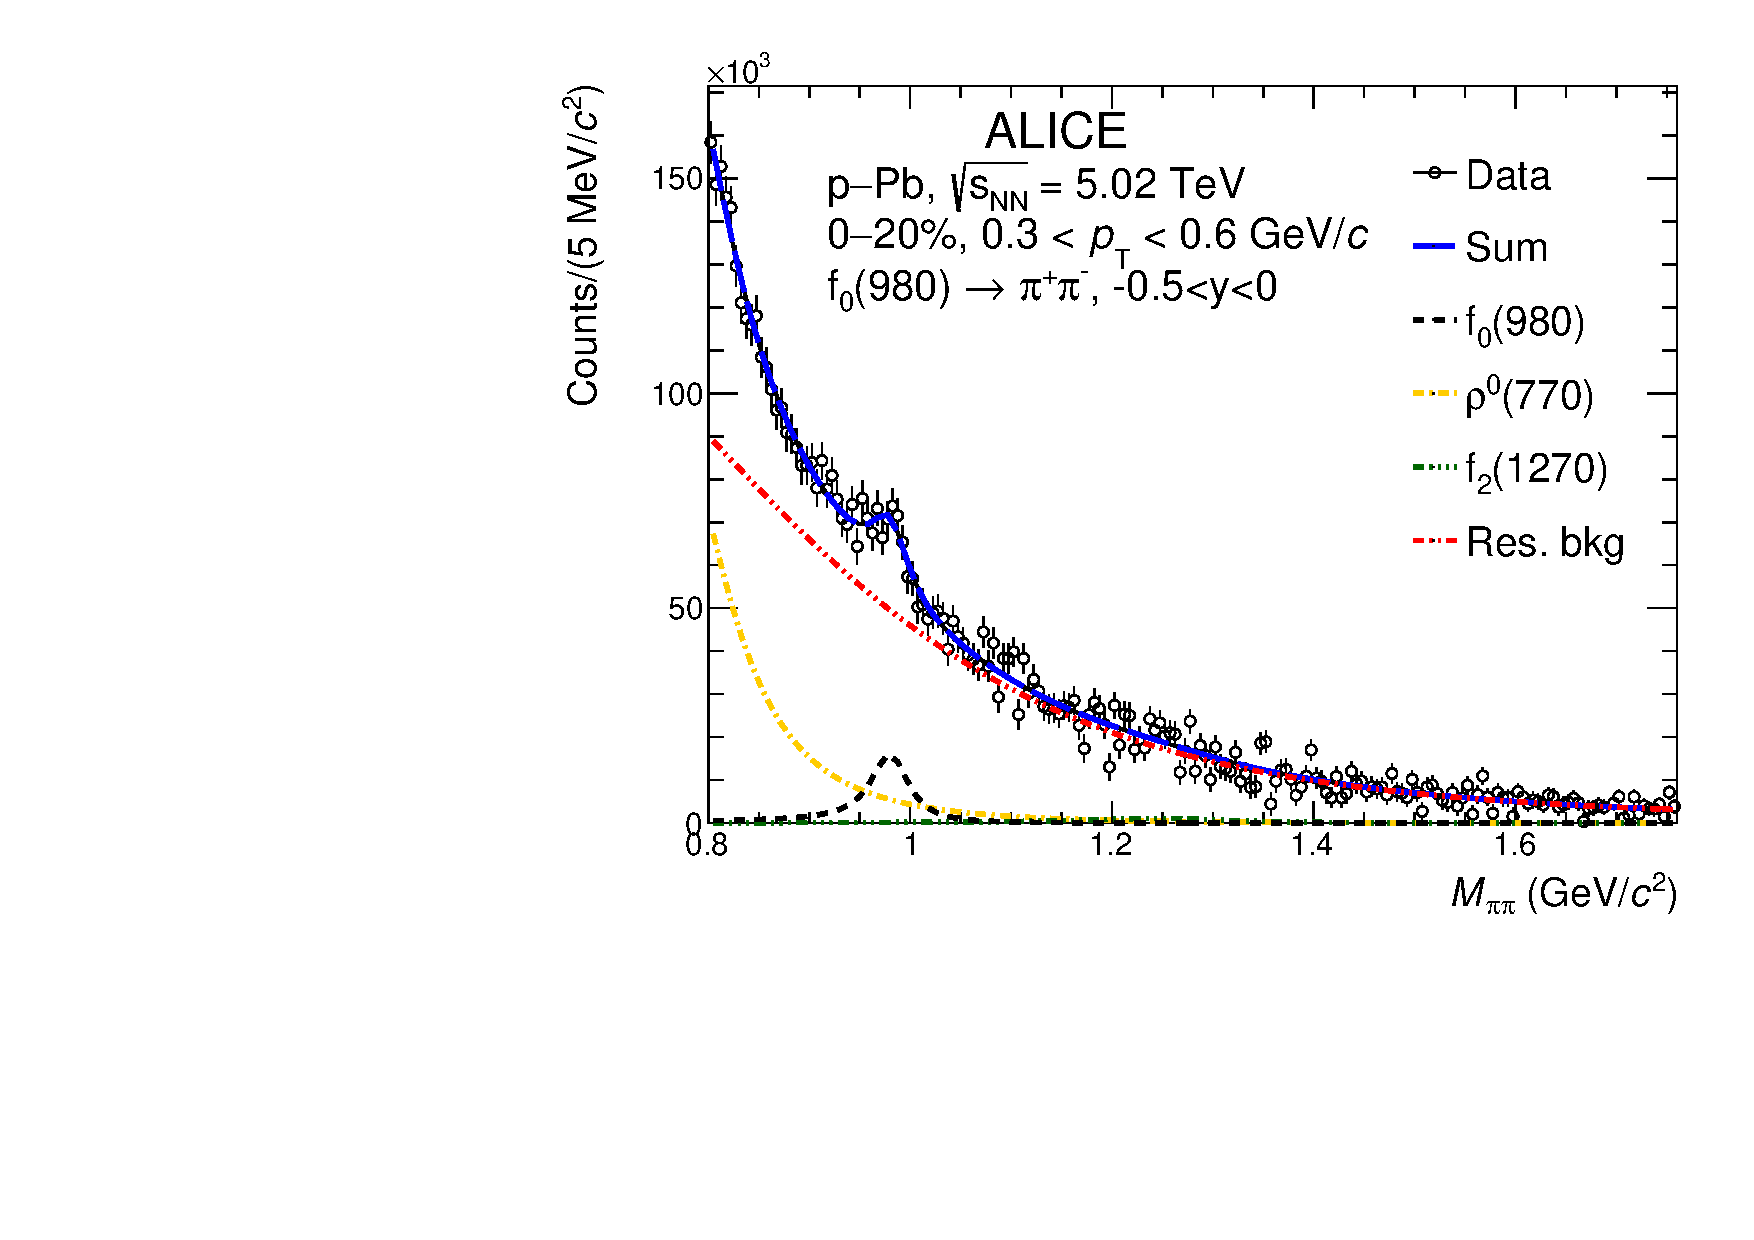
\includegraphics[width=0.47 \textwidth]{figures/Fig1_sigext_high_0pt.pdf} }
	\subfigure{ 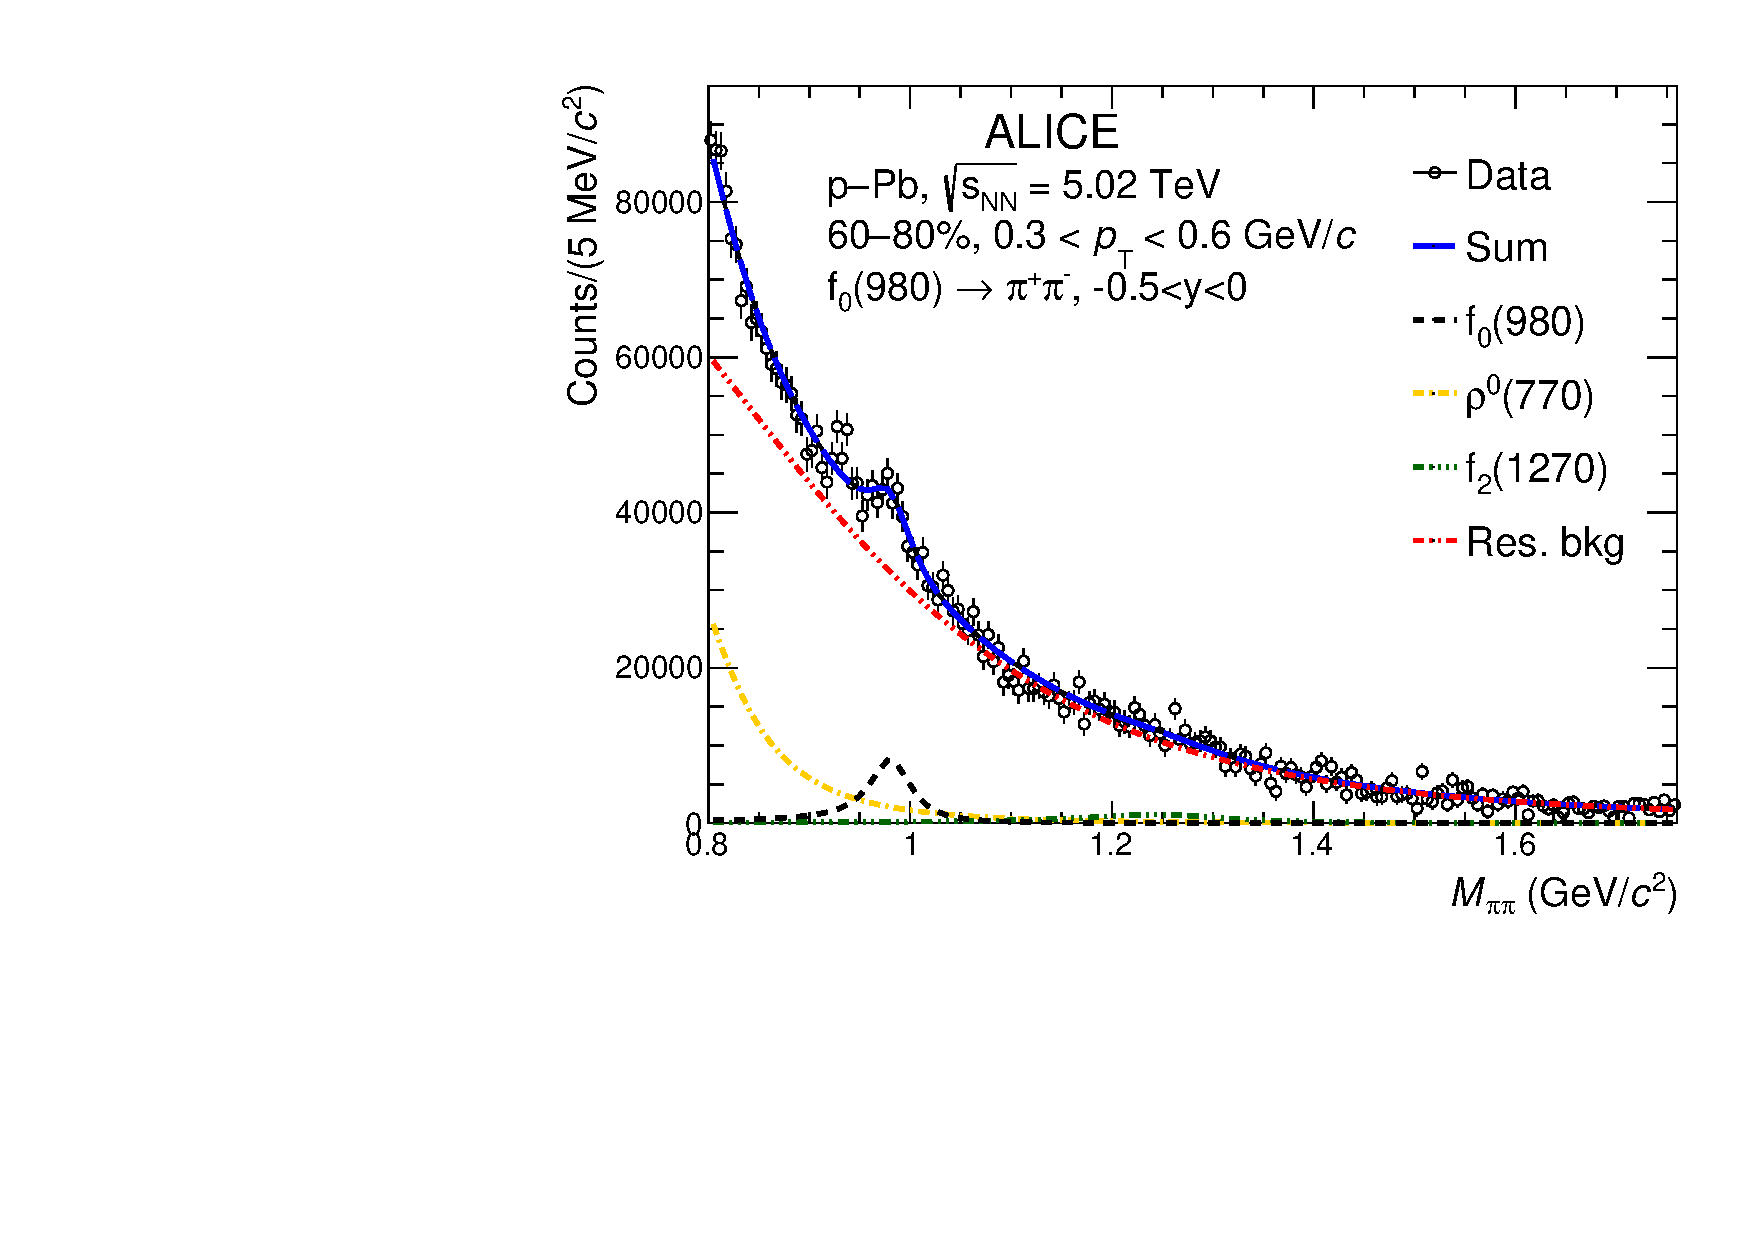
\includegraphics[width=0.47 \textwidth]{figures/Fig1_sigext_low_0pt.pdf} }
	
	\subfigure{ 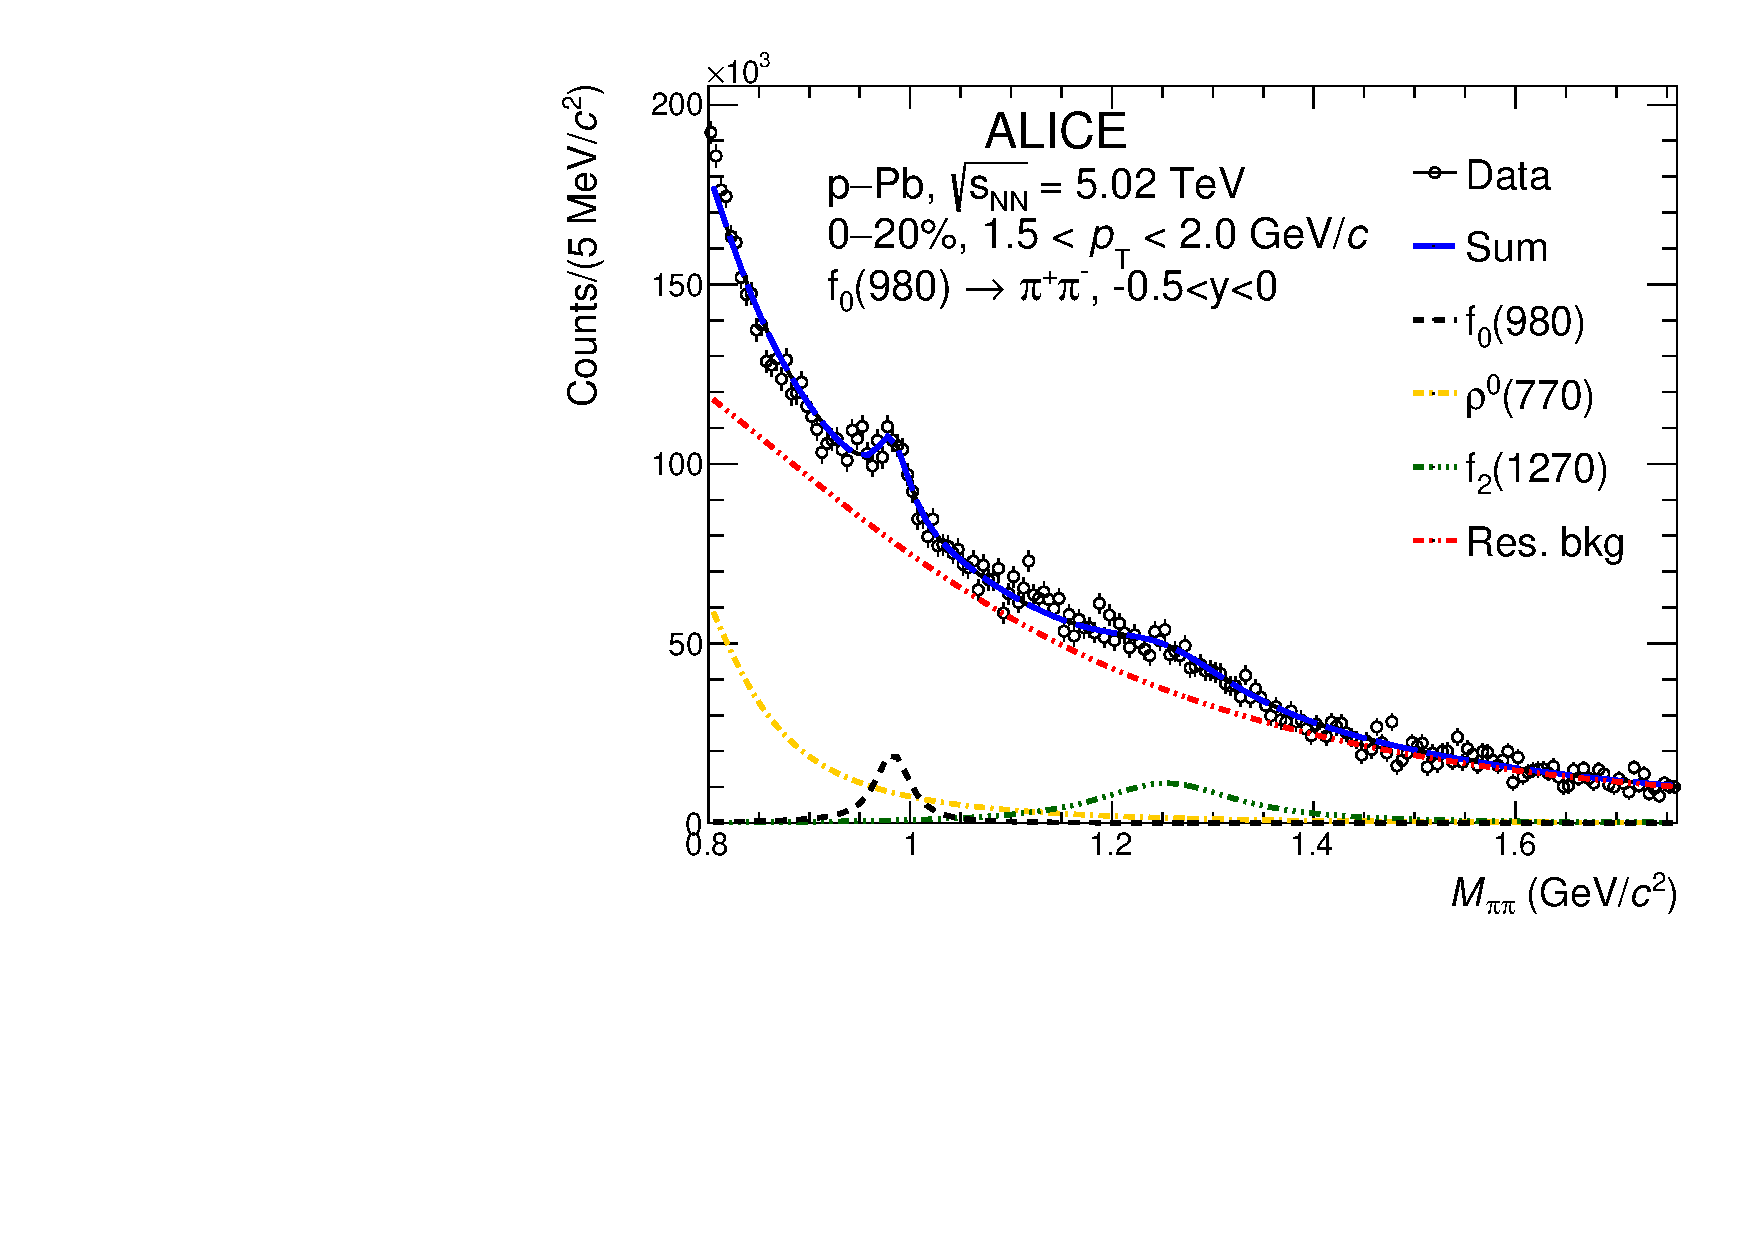
\includegraphics[width=0.47 \textwidth]{figures/Fig1_sigext_high_1pt.pdf} }
	\subfigure{ 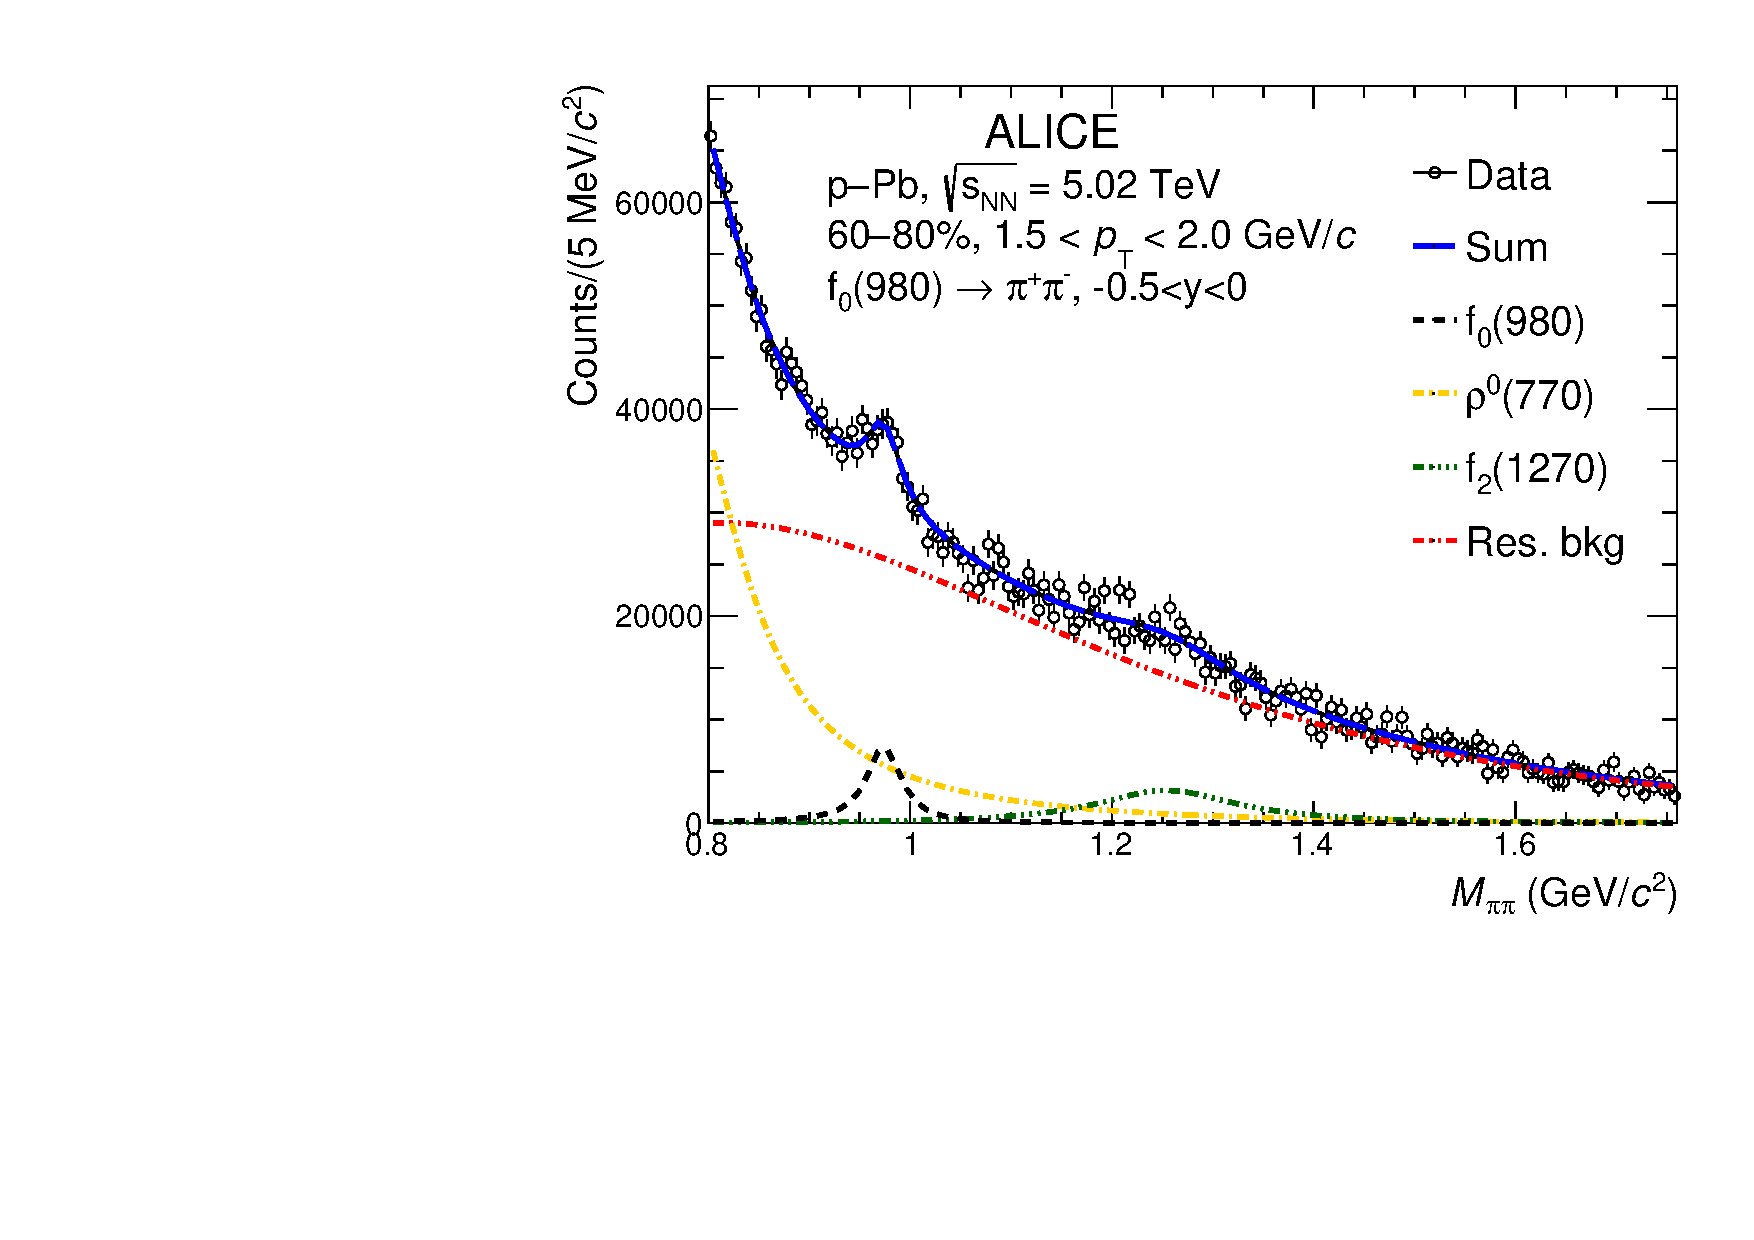
\includegraphics[width=0.47 \textwidth]{figures/Fig1_sigext_low_1pt.pdf} }
	
	\subfigure{ 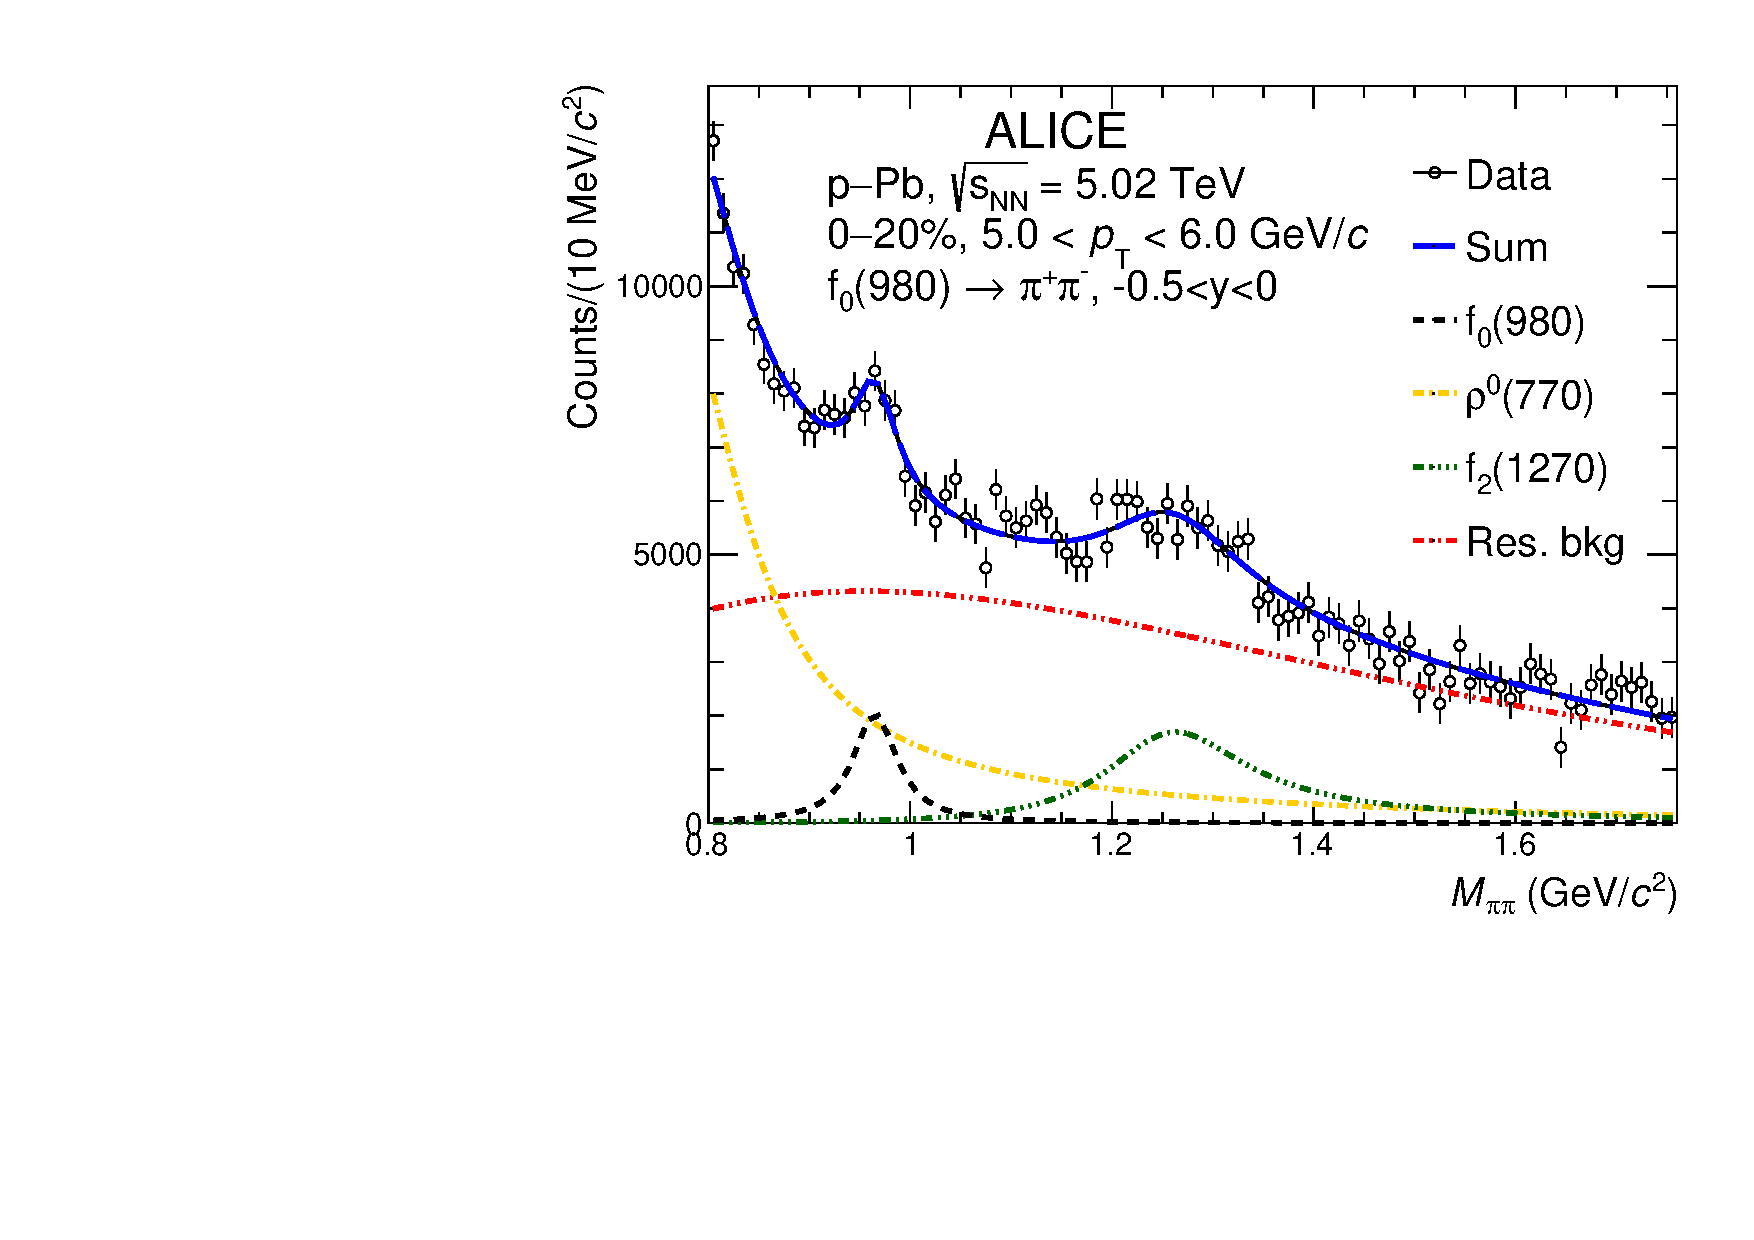
\includegraphics[width=0.47 \textwidth]{figures/Fig1_sigext_high_2pt.pdf} }
	\subfigure{ 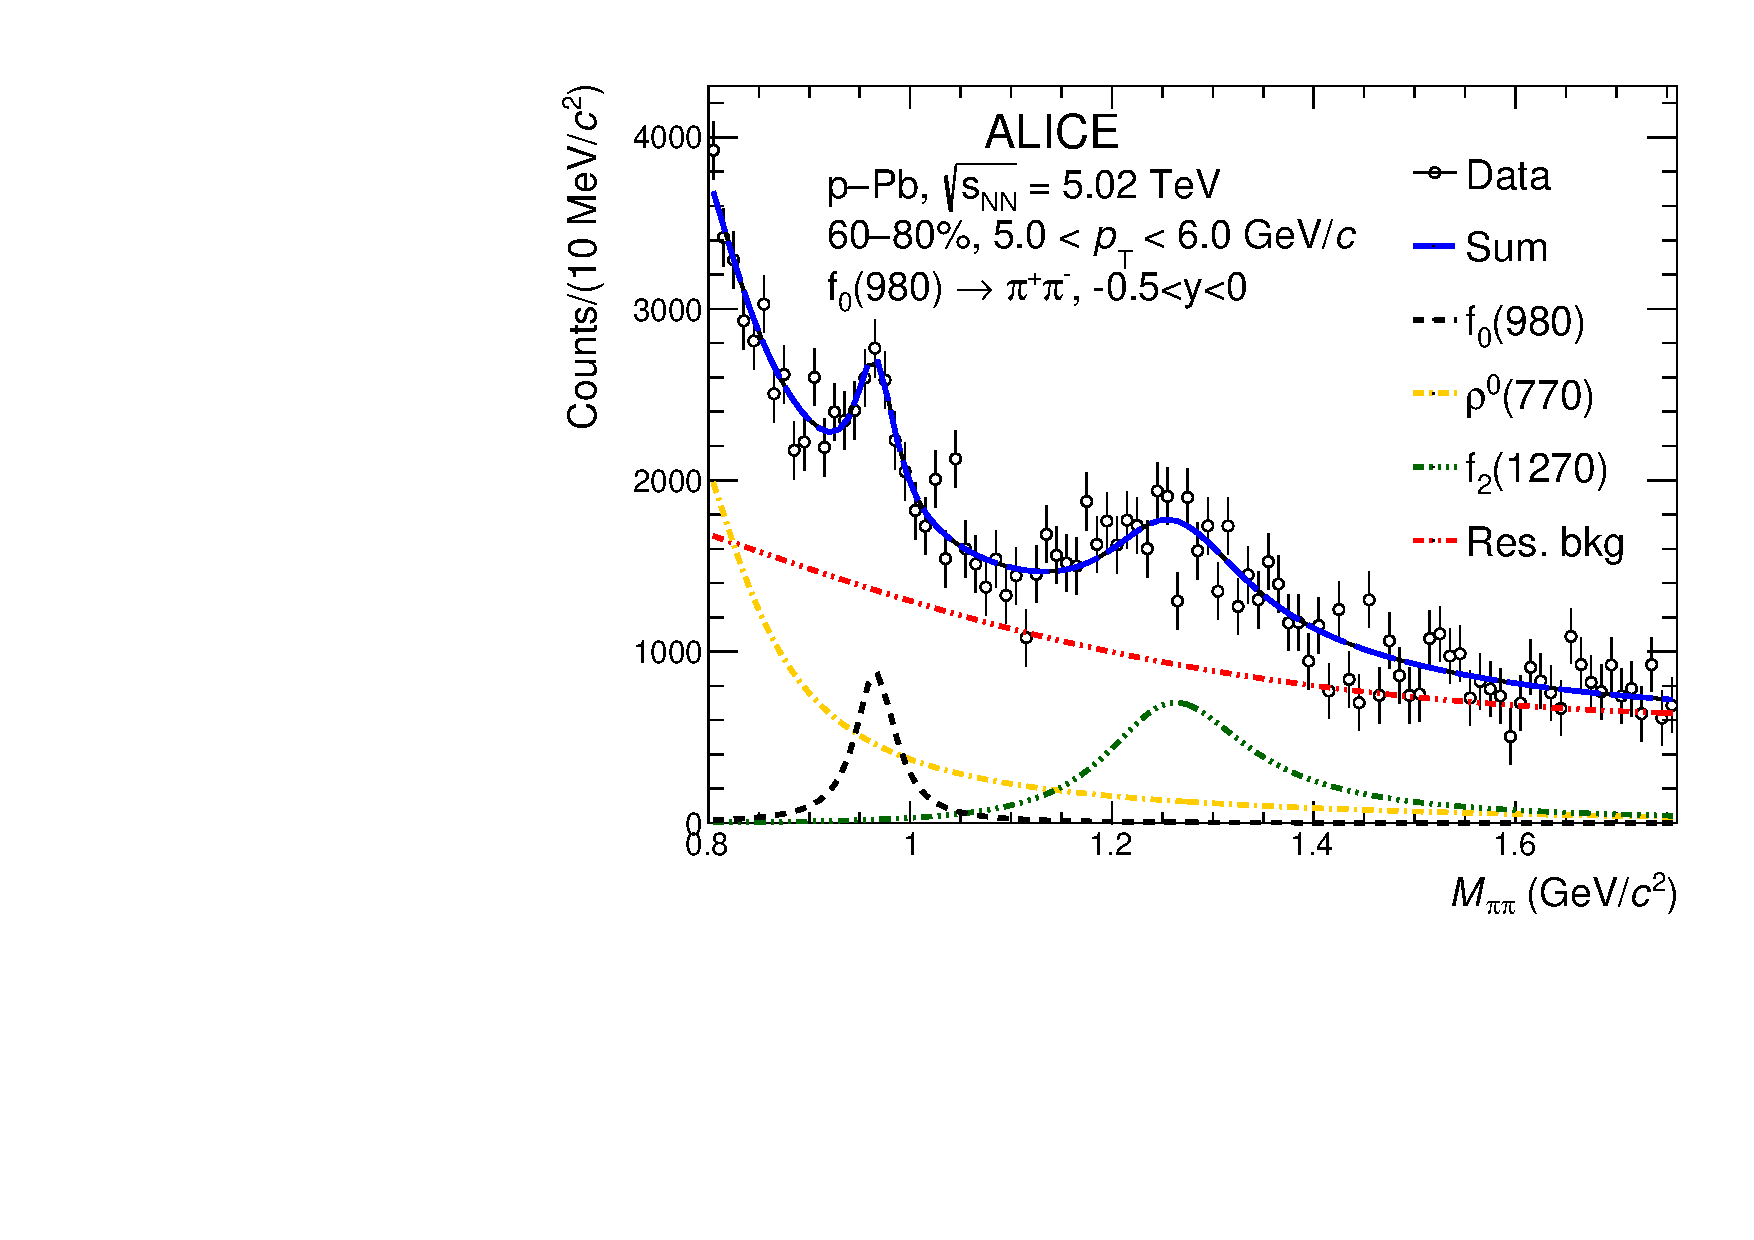
\includegraphics[width=0.47 \textwidth]{figures/Fig1_sigext_low_2pt.pdf} }
	\caption{ Invariant mass distribution of $\pi^{+}\pi^{-}$ pairs after Like-Sign backgrounds subtraction in p--Pb collisions at \snn~=~5.02~TeV in -0.5~$<\mathrm{y}<$~0. Left (Right) plots are obtained from high (low) multiplicity events for different $p_{\mathrm{T}}$ ranges. 
	}
	\label{fig:SigExt}
\end{figure}

The \fzero~is a one of short-lived scalar mesons and its decay vertex is hard to be separated from the primary vertex. The \fzero~is reconstructed with decay channel of \fzero~$\rightarrow \pi^{+}\pi^{-}$, where the branching ratio of the decay is 46\%~\cite{Stone:2013eaa}. The reconstructed tracks are required to satisfy selections listed in the previous work~\cite{ALICE:2018qdv}. The identification of charged pions is done with the TPC and the TOF information. The difference of ionization energy loss between the prediction Bethe-Block parametrization with the pion mass and measured energy is required to be within two standard deviations to identify pions. The difference of flight time between the prediction with the pion mass and measured time is required to be within three standard deviations to identify pions. Identified charged pions are required to be $p_{\rm{T}}>$~0.15~GeV/$c$ and $|\eta|<$~0.8 for a uniform detector acceptance. The pair of two charged pions is required to be -0.5~$<\mathrm{y}<$~0, where $\mathrm{y} = -\mathrm{y}_{\mathrm{lab}} -0.465$~\cite{ALICE:2017pgw}. The combinatorial backgrounds are subtracted with the Like-Sign method~\cite{PhysRevD.36.2019}, which pairs two same charge pions, $\pi^{+}\pi^{+}$ and $\pi^{-}\pi^{-}$. The Like-Sign backgrounds are constructed as the geometric average of $\pi^{+}\pi^{+}$ and $\pi^{-}\pi^{-}$ distributions,  2$\sqrt{N^{\pi^{+}\pi^{+}}N^{\pi^{-}\pi^{-}}}$. After subtracting the Like-Sign backgrounds from $\pi^{+}\pi^{-}$ distribution, peaks of resonances decaying to $\pi^{+}\pi^{-}$ can be seen. Figure~\ref{fig:SigExt} shows the Like-Sign-subtracted $\pi^{+}\pi^{-}$ invariant mass distributions in high-multiplicity (left) and low-multiplicity (right) events for different $p_{\mathrm{T}}$ ranges. Because $\rho$(770) and $\rm{f}_{2}$(1270) dominantly decay to $\pi^{+}\pi^{-}$, \fzero~signals are overlapped with contributions from $\rho$(770) and $\rm{f}_{2}$(1270). Additional backgrounds are attributed to misidentified particles and mini-jets, which are represented as red-dashed-dotted lines in Fig.~\ref{fig:SigExt}. Each resonance contribution is described with relativistic Breit-Wigner function (rBW)~\cite{ALICE:2018qdv, ALICE:2022qnb} because detector resolution is expected to be negligible with respect to the particle width. The rBW can be expressed as
\begin{eqnarray}
\mathrm{rBM}(M_{\pi\pi}) = \dfrac{AM_{\pi\pi}\Gamma(M_{\pi\pi})M_{0}}{(M_{\pi\pi}^{2}-M_{0}^{2})^{2} + M_{0}^{2}\Gamma^{2}(M_{\pi\pi})},
\label{eq:rBW}
\end{eqnarray}
where $\Gamma(M_{\pi\pi})$ is
\begin{eqnarray}
\Gamma(M_{\pi\pi}) = \left[ \dfrac{ (M_{\pi\pi}^{2} - 4m_{\pi}^{2}) }{ (M_{0}^{2}-4m_{\pi}^{2}) } \right]^{(2J+1)/2} \times \dfrac{\Gamma_{0}M_{0}}{M_{\pi\pi}}
\label{eq:rBWW}
\end{eqnarray}
$A$ and $M_{0}$ in eq~\ref{eq:rBW} are amplitude of the rBW and  the rest mass of the resonance, respectively. $\Gamma_{0}$, $J$, and $m_{\pi}$ the are rest width of the resonance, the spin, and the charged pion mass, respectively. The spin for \fzero~, $\rho$(770), and $\mathrm{f}_{2}$(1270) are 0, 1, and 2, respectively. Residual backgrounds ($f_{\mathrm{bkg}}$) is expressed with a similar function with the Maxwell-Boltzmann distribution, which can be expressed as~\cite{OPAL:1998enc}
\begin{eqnarray}
f_{\mathrm{bkg}}(M_{\pi\pi}) = B(M_{\pi\pi}-2m_{\pi})^{n}\exp{(c_{1}M_{\pi\pi} + c_{2}M_{\pi\pi}^{2})}.
\label{eq:bkg}
\end{eqnarray} 
Each rBW of the resonance is corrected for phase space, a mass dependent reconstruction efficiency and $\pi\pi$ interference as described by~\cite{Rapp:2003ar}, which can be expressed as
\begin{eqnarray}
\mathrm{PS}(M_{\pi\pi}) = \dfrac{M_{\pi\pi}}{\sqrt{M_{\pi\pi}^{2}+p_{\mathrm{T}}^{2}}}\times\exp{(-\sqrt{M_{\pi\pi}^{2}+p_{\mathrm{T}}^{2}})},
\label{eq:ps}
\end{eqnarray} 
where $T$ is the kinetic freeze-out temperature and set to 160~MeV~\cite{ALICE:2013wgn} for different multiplicity classes.

The signal extraction carefully considers the width of \fzero~as the width is not constrained (10~$<\Gamma_{\mathrm{f}_{0}}<$~100~MeV/$c^{2}$~\cite{ParticleDataGroup:2020ssz}). Total fit function consists of three rBWs and $f_{\mathrm{bkg}}$, which is constructed with 9 fit parameters as the masses and widths of $\rho$(770) and $\mathrm{f}_{2}$(1270) are well defined in~\cite{ParticleDataGroup:2020ssz}, and those are fixed. The first fit procedure is only conducted in minimum-bias events for merged $p_{\mathrm{T}}$ ranges to accumulate enough statistics while all parameters are left free to obtain unbiased \fzero~width. The second fit procedure is conducted with the fixed \fzero~width, which is obtained from the first procedure, and no constraints for other parameters. As a result of the second procedure, four parameters of backgrounds function are determined. The last fit procedure is conducted with the fixed background function, and no constraints for other parameters. In each step, the fit range is set to 0.8~$<M_{\pi\pi}<$~1.76~GeV/$c^{2}$. Such multiple steps are designed to prevent fit results from being in local minimum and to minimize possible biases to the estimation of the \fzero~width. 

Raw \fzero~yields from fit procedures are corrected for the acceptance and the tracking efficiency, and normalized for the event selections and the branching fraction~\cite{ALICE:2022qnb}. Coefficients for the accepance and the tracking efficiency are estimated from a detailed simulation for the ALICE detector responses. The p--Pb events are simulated using the DPMJET~\cite{Fedynitch:2015kcn} event generator with the artificial injection of \fzero~signals. The generated \fzero~are transported through the detector using GEANT3~\cite{Brun:1994aa}. The acceptance multiplied by the tracking efficiency is estimated to be 26\% and gradually increasing up to 60\% as $p_{\mathrm{T}}$ increases. 

A comparison of the $p_{\rm{T}}$ differential invariant yield between p--Pb and pp collisions, which is called the nuclear modification factor ($Q_{\mathrm{pPb}}$), can be expressed as
\begin{eqnarray}
Q_{\mathrm{pPb}} = \dfrac{\mathrm{d}^{2} N_{\mathrm{f}_{0}(980)}^{\mathrm{pPb}} / \mathrm{d} p_{\mathrm{T}} \mathrm{dy} }{ \left\langle T_{\mathrm{pPb}} \right\rangle \mathrm{d}^{2} \sigma_{\mathrm{f}_{0}(980)}^{\mathrm{pp}}/ \mathrm{d} p_{\mathrm{T}} \mathrm{dy} },
\end{eqnarray}
where $\left\langle T_{\mathrm{pPb}} \right\rangle$ and $\sigma_{\mathrm{f}_{0}(980)}^{\mathrm{pp}}$ are the average nuclear overlap from the Glauber model~\cite{Miller:2007ri} and the cross section of \fzero~in pp collisions~\cite{ALICE:2022qnb}, respectively. 

\section{Systematic uncertainties}
\label{sec:syst}
The systematic uncertainties of invariant yields are estimated by varying the analysis selection criteria and corrections, which are summarized in Tab.~\ref{tab:syst}. Total systematic uncertainty is calculated as a quadrature of each uncertainty.

\begin{table}[h!]
\caption{The relative systematic uncertainty of invariant $p_{\rm{T}}$-differential yields. Numbers given in ranges correspond to minimum and maximum uncertainties.}
\centering
\begin{tabular}{cc|c}
\hline 
\multicolumn{2}{c|}{Sources}  &Systematic uncertainty (\%) \\ \hline
\multicolumn{2}{c|}{Tracking} & $\pm$4--6 \\
\multicolumn{2}{c|}{Particle identification} & $\pm$4--12 \\ 
\multirow{4}{*}{Signal extraction} &  $\mathrm{f}_{2}$(1270) Par.	& $\pm$3--9 \\ 
& $\rho$(770) Par. & $\pm$3--8 \\
& Fit range & $\pm$0--6 \\
& Init. $\mathrm{f}_{0}$ width & $\pm$2--12 \\
\multicolumn{2}{c|}{Phase space correction} & $\pm$3--8 \\ \hline 
\multicolumn{2}{c|}{Total (in quadrature)}	& $\pm$15--27 \\ 
\hline 
\end{tabular}
\label{tab:syst}
\end{table}

The systematic uncertainty from the primary vertex selection is tested by narrowing the requirement to 7~cm and the uncertainty is estimated to be negligible. The systematic uncertainty from the pileup rejection is tested by varying the minimal number of track contributors required for reconstruction of pileup event vertices from 5 to 3 and the uncertainty is estimated to be negligible.

The systematic uncertainty from tracking is assigned as the value from~\cite{ALICE:2013wgn} and the systematic uncertainty from the particle identification is tested with different requirements on the number of standard deviations by $\pm\,0.5\sigma$ for the TPC and the TOF, and the uncertainties are estimated to be 4--12\%.

The systematic uncertainties from masses and widths of $\mathrm{f}_{2}$(1270) and $\rho$(770) are evaluated by shifting the masses and the widths as much as three times their measured statistical uncertainty. The estimated uncertainties from $\mathrm{f}_{2}$(1270) and $\rho$(770) parameters are 3--9\% and 3--8\%, respectively. The systematic uncertainty from the fit range is estimated by changing the range inward or outward as much as 40~MeV/$c^{2}$. The uncertainties are estimated to be 0--6\%.

The systematic uncertainty from the initial \fzero~width, which is obtained in the first fit procedure and used in the second fit procedure (see Sec.~\ref{sec:ana}), is estimated by varying the width as much as their measured statistical uncertainty in both directions. The estimated systematic uncertainties are 2--12\%.

The systematic uncertainty from phase space correction is estimated by varying the kinetic freeze-out temperature in the range of 140~$<T_{\mathrm{kin}}<$~180~MeV. The estimated uncertainty is 3--8\%. 

\begin{comment}
The systematic uncertainties of invariant yields and \fzero~widths are estimated by varying the analysis selection criteria and corrections, which are summarized in Tab.~\ref{tab:syst}.

The systematic uncertainty from the primary vertex selection is tested by narrowing the requirement to 7~cm and the uncertainty is estimated to be negligible. The systematic uncertainty from the pileup rejection is tested by varying the minimal number of track contributors required for reconstruction of pileup event vertices from 5 to 3 and the uncertainty is estimated to be negligible.

The systematic uncertainty from tracking is assigned as the value from~\cite{ALICE:2013wgn} and the systematic uncertainty from the particle identification is tested with different requirements on the number of standard deviations by $\pm\,0.5\sigma$ for the TPC and the TOF, and the uncertainties are estimated to be 4--12\% for invariant yield and 5--10\% for width.

The systematic uncertainties from masses and widths of $\mathrm{f}_{2}$(1270) and $\rho$(770) are evaluated by shifting the masses and the widths as much as three times their measured statistical uncertainty. The estimated uncertainties for $\mathrm{f}_{2}$(1270) ($\rho$(770)) parameters are 3--9\% (3--8\%) and 2--7\% (2--8\%) for the mass and the width, respectively. The systematic uncertainty from the fit range is estimated by changing the range inward or outward as much as 40~MeV/$c^{2}$. The uncertainties are estimated to be 0--6\% for the yield and 0--5\% for the width.

On the other hand, the width of \fzero~is loosely defined so that \fzero~width is set to free parameter and estimated in the fit procedure. The systematic uncertainty from the fit range is tested with different fit ranges and estimated to be 2\% at the low $p_{\rm{T}}$ and 8\% at the high $p_{\rm{T}}$. The phase space correction~\cite{Rapp:2003ar} is applied to each rBW to consider possible $\pi\pi$ scattering effects. The temperature of the phase space correction is set to 160 MeV~\cite{ALICE:2013wgn} and the systematic uncertainty from the phase space correction is evaluated with different temperatures and estimated to be 5--7\%. The background function is determined with the pre-fit procedure. In the pre-fit procedure, the width of \fzero~is even fixed as a specific value. The systematic uncertainty from the background function is evaluated with different \fzero~widths and estimated to be 8\% at the low $p_{\rm{T}}$ and 3\% at the high $p_{\rm{T}}$.
\end{comment}